%!TEX root = ../pres - final.tex

\section{Modelos de Markov}
\subsection{Hidden Markov Model}
\begin{frame}{Cadenas de Markov}
    \begin{itemize}
      \itemsep2em
      \item Cadena de Markov de primer orden      
        \\~\\
        \begin{center}
          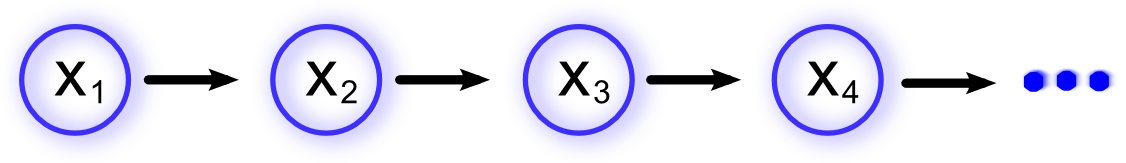
\includegraphics[width=0.4\textwidth]{gfx/mod-mm1}
        \end{center}        
        \begin{equation}
          \label{eqn:2-4}
          p(x_1, ..., x_T) 
            ~=~ \prod_{t=1}^T p(x_T ~|~ x_1, ..., x_{t-1}) 
            ~=~ p(x_1) \cdot \prod_{t=2}^T p(x_T ~|~ x_{t-1}) 
        \end{equation} 
      \item  Se puede generalizar para cadenas de Markov de un orden mayor
        \\~\\
        \begin{center}
          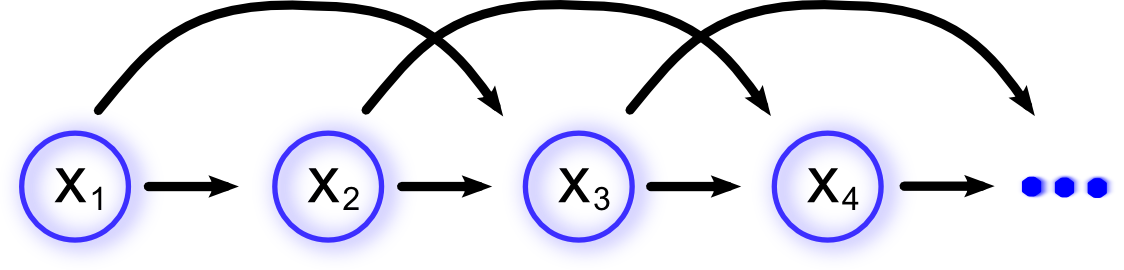
\includegraphics[width=0.45\textwidth]{gfx/mod-mm2}
        \end{center}
        \begin{equation}
          \label{eqn:2-4}
          p(x_1, ..., x_T) 
            ~=~ p(x_1) p(x_2 ~|~ x_1) \cdot \prod_{t=3}^T p(x_T ~|~ x_{t-1}, x_{t-2}) 
        \end{equation} 
  \end{itemize} 
\end{frame}

\begin{frame}{Modelo oculto de Markov}
  \begin{itemize}
    \itemsep1em
    \item Agregar una variable latente $z_t$ (discreta), que corresponda a cada observación $x_t$.
      \begin{align}
        z_{t+1} &\perp z_{t-1} ~|~ z_{t} \\
        p(x_1, ..., x_T, z_1, ..., z_T) &~=~ p(z_1) \left [ \prod_{t=2}^T p(z_t ~|~ z_{t-1}) \right ] 
          \prod_{t=1}^T p(x_t ~|~ z_{t}).
      \end{align}

    \item Modelar proceso bivariado en el tiempo. Una variable observada y una variable latente asociada.
      \\~\\
      \begin{center}
        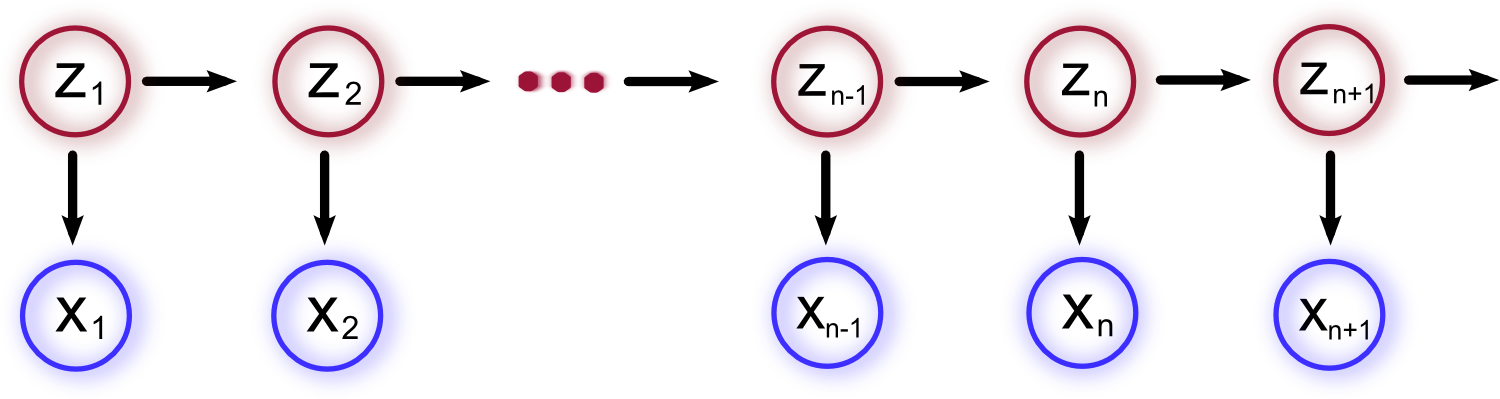
\includegraphics[width=0.5\textwidth]{gfx/mod-hmm}
      \end{center}    
      
    \item Mezcla de distribuciones en la que la densidad está dada por $p(x | z)$      
  \end{itemize}
\end{frame}

\begin{frame}{Parámetros del HMM}
  \begin{itemize}
    \item Probabilidad de cambio entre estados dada una \alert{matriz de transición} $\mathbf{A}$
      \begin{align}
        A_{jk} &\equiv p(z_{tk} = 1 ~|~  z_{t-1, j} = 1) \\
        p(z_t ~|~ z_{t-1}, \mathbf{A}) &= \prod_{k=1}^K \prod_{j=1}^K A_{jk}^{z_{{n-1}, j} \cdot z_{t,k}}
      \end{align}      
    \item \alert{Vector de distribución inicial} $\bm{\pi}$ para variable latente.
      \begin{align}
        \pi_k &\equiv p(z_{1k}) \\
        p(z_1 ~|~ \pi) &= \prod_{k=1}^K \pi_k^{z_{1k}}
      \end{align}       
    \item \alert{Probabilidad de emisión} de una variable observada $x_t$ dada una variable latente $z_t$.
      \begin{equation}
        p(x_t ~|~ z_t, \phi) = \prod_{k=1}^K p(x_t ~|~ \phi_k) ^ {z_{tk}}
      \end{equation}
  \end{itemize}
\end{frame}

\begin{frame}{Parámetros del HMM}
  \begin{itemize}
    \itemsep1em
    \item \alert{Probabilidad conjunta del modelo}
      \begin{equation}
        p(\mathbf{X}, \mathbf{Z} ~|~ \theta)        
          = p(z_1 ~|~ \pi) \left[ \prod_{t=2}^T p(z_t ~|~ z_{t-1}, \mathbf{A}) \right]
          \prod_{t=1}^T p(x_t ~|~ z_t, \mathbf{B}, \phi)
      \end{equation}      
      donde $\mathbf{X} = \lbrace x_1, ..., x_N \rbrace$,~ $\mathbf{Z} = \lbrace z_1, ..., z_N \rbrace$ \\
      y los parámetros del modelo son $\theta = \lbrace \bm{\pi}, \mathbf{A}, \mathbf{B}, \phi \rbrace$

    \item Es difícil determinar los parámetros del HMM por Máxima Verosimilitud, pues la función de verosimilitud es 
      \begin{equation}
        p(\mathbf{X}, \theta) = \sum_Z p(\mathbf{X}, \mathbf{Z} \,|\, \theta)
        \label{eqn:3-1}
      \end{equation}
  \end{itemize}
\end{frame}    

\subsection{Resolver HMM con EM}

\begin{frame}{Estimación de parámetros de HMM con EM}
  \begin{itemize}      
    \itemsep1em
    \item Si en vez de usar la función de verosimilitud \eqref{eqn:3-1}, consideramos la verosimilitud de los datos completos $p(\mathbf{X}, \mathbf{Z})$, la maximización de esta función sería mucho más directa.

    \item No se conocen los datos completos $\lbrace \mathbf{X}, \mathbf{Z} \rbrace$.

    \item Utilizar el algoritmo EM para maximizar de forma eficiente la función de verosimilitud del HMM.
    \item Se propone usar la función de verosimilitud completa, y maximizar la esperanza 
      del logaritmo de ésta.
      \begin{equation}
        \mathcal{Q}(\theta, \theta^{old}) 
             = \mathbb{E}_{\mathbf{Z} | \theta^{old}} 
             \left[ \log p(\mathbf{X}, \mathbf{Z} \,|\, \theta) \right]       
      \end{equation}
      \\~\\
      \begin{equation}
        \mathcal{Q}(\theta, \theta^{old}) 
            = \sum_{\mathbf{Z}} p(\mathbf{Z} ~|~ \mathbf{X}, \theta^{old})
              \log p(\mathbf{X}, \mathbf{Z} ~|~ \theta)
      \end{equation}
      \vspace{.5em}      
  \end{itemize}
\end{frame}

\begin{frame}{Estimación de parámetros de HMM con EM}{Notación}  
  Se utilzará la siguiente notación para simiplificar el desarrollo: \\~\\
  \begin{description}
        \item[Probabilidad marginal de una variable latente]
          \begin{equation}
            \gamma(z_t) = p(z_t ~|~ \mathbf{X}, \theta^{old})
            \label{eqn:3-3}
          \end{equation}

        \item[Probabilidad conjunta de dos variables latentes consecutivas]
          \begin{equation}
            \xi(z_{t-1}, z_T) = p(z_{t-1}, z_T ~|~ \mathbf{X}, \theta^{old})
            \label{eqn:3-4}
          \end{equation}
      \end{description}
      donde
      \begin{align}
        \gamma(z_{tk}) &= \mathbb{E} \left[ z_{tk} \right] = 
                \sum_Z  \gamma(\mathbf{z}) \cdot z_{tk} \label{eq-13} \\
        \xi(z_{t-1,j}, z_{tk}) &= \mathbb{E} \left[z_{t-1, j} \cdot z_{tk} \right] = 
          \sum_Z  \gamma(\mathbf{z}) z_{t-1, j} \cdot z_{tk} \label{eq-14}
      \end{align}  
      
      %\item Prob. marginal de $z_{tk} = 1$, prob. conjunta de $z_{t-1,j}, z_{tk}$
\end{frame}

\begin{frame}{Estimación de parámetros de HMM con EM}{E-Step}
  \begin{itemize}
    \item Función de verosimilitud completa (reescrita con \eqref{eq-13}, \eqref{eq-14})
      \begin{equation}
        \begin{split}
          \mathcal{Q}(\theta, \theta^{old}) = 
          \sum_{k=1}^K \gamma(z_{1k}) \log \pi_k + 
          \sum_{t=2}^T \sum_{j=1}^K \sum_{k=1}^K \xi(z_{t-1,j}, z_{tk}) \log A_{jk} + \\
          \sum_{t=1}^T \sum_{k=1}^K \gamma(z_{tk}) \log p(x_T ~|~ \phi_k)
        \end{split}
      \end{equation}
  \end{itemize}
\end{frame}          

\begin{frame}{Estimación de parámetros de HMM con EM}{M-Step}          
  \begin{itemize}
     \itemsep1.5em
     \item $\theta_{new} = \underset{\theta}{arg~max}~\mathcal{Q}(\theta, \theta^{old})$
     \item Parámetros estimados por EM: 
     \begin{equation}
       \pi_k = \frac{\gamma(z_{1k})}{\sum_{j=1}^K \gamma(z_1j)}, ~~
       A_{jk} = \sum_{t=2}^T \frac{\xi(z_{t-1,j}, z_{tk})}{ \sum_{l=1}^K \xi(z_{t-1,j}, z_{tl})}
     \end{equation}
  \end{itemize}
\end{frame}

\subsection{Algoritmo backward-forward}
\label{sec:algoritmo_backward_forward}

\begin{frame}{Algoritmo backward-forward}
  \begin{align}
  \gamma(z_t) &= p(z_t ~|~ X) = \frac{p(X ~|~ z_t) p(z_t)}{p(X)} \\
  \gamma(z_t) &= \frac{p(x_1, ..., x_t, z_t)p(x_{t+1}, ..., x_T ~|~ z_t)}{p(X)} \\
  \gamma(z_t) &= \frac{\alpha(z_t) \beta(z_t)}{p(X)} \\  
  \end{align}
  donde 
  \begin{align}
    \alpha(z_t) &\equiv p(x_1, ..., x_t, z_t) \\
    \beta(z_t) &\equiv p(x_{t+1}, ..., x_T ~|~ z_t)    
  \end{align}  
\end{frame}

\begin{frame}{Algoritmo backward-forward}
  \begin{align}
    \alpha(z_t) &= p(x_t ~|~ z_t) \sum_{z_{t-1}} \alpha(z_t ~|~ z_{t-1}) 
    \label{eqn:3-15}
    \\ 
    \alpha(z_1) &= p(z_1) p(x_1 ~|~ z_1) = \prod_{k=1}^K \lbrace {\pi_k p(x_1 ~|~ \phi_k)} \rbrace ^ {z_{1k}} 
    \\ 
    \notag \\ 
    \beta(z_t) &= \sum_{z_{t+1}} \beta(z_{t+1})p(x_{t+1} ~|~ z_{t+1}) p(z_{t+1} ~|~ z_t) \\ 
    \beta(z_T) &= 1
  \end{align}  
\end{frame}

\begin{frame}{Factor de escala}
  \begin{itemize}
    \itemsep1em

    \item En el proceso recursivo para calcular cada $\alpha(z_n)$ se utilizan las \structure{probabilidades} $\alpha(z_{n-1})$ anteriores...

    \item Manejar las probabilidades de forma re-escalada.
      \begin{equation}
        \hat \alpha(z_n) = p(z_n \,|\, x_1, ..., x_n )
            = \frac{\alpha(z_n)}{p(x_1, ..., x_n)}
          \label{eqn:3-21}
      \end{equation}

    \item Se puede introducir un término de escala para cada $\hat \alpha(z_n)$
      \begin{equation}
        c_n = p(x_n \,|\, x_1, ..., x_{n-1})
        \label{eqn:3-22}
      \end{equation}
    por lo que entonces
      \begin{equation}
        p(x_1, ..., x_n) = \prod_i^n c_i 
        \label{eqn:3-23}
      \end{equation}
  \end{itemize}
\end{frame}

\begin{frame}{Factor de escala}{$\alpha$}
  \begin{itemize}
    \itemsep1em    
    \item A partir de \eqref{eqn:3-21} y \eqref{eqn:3-23} se puede escribir $\alpha(z_n)$ como sigue: 
    \begin{align}
      \alpha(z_n) &= p(x_1, ..., x_n, z_n) \notag \\
        &= \left( \prod_i^n c_i \right) \hat \alpha(z_n)    
      \label{eqn:3-24}
    \end{align}
  y entonces la forma recursiva \eqref{eqn:3-15} se puede reescribir
    \begin{equation}
      c_n \hat \alpha(z_n) = p(x_n \,|\, z_n) \sum_{z_{n-1}} 
        \hat \alpha(z_{n-1}) p(z_n \,|\, z_{n-1})
        \label{eqn:3-25}
    \end{equation}
  \end{itemize}
\end{frame}

\begin{frame}{Factor de escala}{$\beta$}
  \begin{itemize}
    \itemsep1em    
    \item Para re-escalar $\beta(z_n)$ usando los coeficientes $c_n$ se tiene
      \begin{equation}
        \beta(z_n) = \left( \prod_i^n c_i \right) \hat \beta(z_n)
        \label{eqn:3-26}
      \end{equation}
    donde 
      \begin{equation}
        \hat \beta(z_n) = 
          \frac{p(x_{n+1}, ..., x_N \,|\, z_n)}
          {p(x_{n+1}, ..., x_N \,|\, x_1, ..., x_n)}
        \label{eqn:3-27}
      \end{equation}
    a partir de lo cual se puere escribir
      \begin{equation}
        c_{n+1} \hat \beta(z_n) = \sum_{z_{n+1}} \hat \beta(z_{n+1})
          p(x_{n+1} \,|\, z_{n+1}) p(z_{n+1} \,|\, z_n)    
        \label{eqn:3-28}
      \end{equation}
  \end{itemize}
\end{frame}    

\begin{frame}{Factor de escala}{$\gamma$, $\xi$}
  \begin{itemize}
    \itemsep1em    
    \item Y entonces tanto \eqref{eqn:3-3} como \eqref{eqn:3-4} se pueden formular de la siguiente manera: 
      \begin{align}
        \gamma(z_n) &= \hat \alpha(z_n) \hat \beta(z_n) \\
        \xi(z_{n-1}, z_n) &= c_n \hat \alpha(z_{n-1}) p(x_n \,|\, z_n) 
            p(z_n \,|\, z_{n-1}) \hat \beta(z_n) 
        \label{eqn:3-30}      
      \end{align}
    \end{itemize}
\end{frame}    

\begin{frame}{Secuencia recuperada}
  \begin{itemize}
    \itemsep1em    
    \item 
    Como menciona Rabiner \cite{Rabiner1989}, hay muchas formas en las que se puede definir la secuencia óptima.

    \item
     Escoger las probabilidades marginales de las variables latentes $\gamma(z_n)$ \eqref{eqn:3-8} más probables de forma individual:
    \begin{equation}
    q_k = \underset{1 <= k <= K}{arg~max}~ \gamma(z_{nk}), \quad \quad 1 <= n <= N
    \label{eqn:3-31}
    \end{equation}

    \item
    Otra opción, puede ser usar el algoritmo de Viterbi que nos permite obtener la secuencia de estados más probable dada una secuencia observada. 
  \end{itemize}
\end{frame}